% z2xz3.tex

\documentclass[tikz]{standalone}
\usetikzlibrary{positioning}

\begin{document}
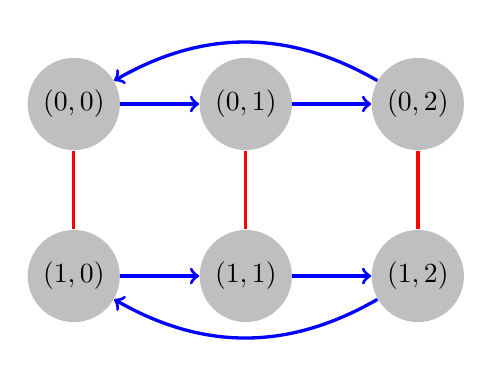
\begin{tikzpicture}[ele/.style = {circle, minimum size = 8pt, fill = lightgray},
  op/.style = {->, blue, very thick}]
  % (0, )
  \node (00) [ele] {$(0, 0)$};
  \node (01) [ele, right = of 00] {$(0, 1)$};
  \node (02) [ele, right = of 01] {$(0, 2)$};

  \path (00) edge[op] (01)
		(01) edge[op] (02)
		(02) edge[op, bend right] (00);

  % (1, )
  \node (10) [ele, below = of 00] {$(1, 0)$};
  \node (11) [ele, right = of 10] {$(1, 1)$};
  \node (12) [ele, right = of 11] {$(1, 2)$};

  \path (10) edge[op] (11)
		(11) edge[op] (12)
		(12) edge[op, bend left] (10);

  % (0, ) -- (1, )
  \foreach \y in {0, 1, 2} {
	\draw[-, red, very thick] (0\y) to (1\y);
  }
\end{tikzpicture}
\end{document}
